%++++++++++++++++++++++++++++++++++++++++
% Don't modify this section unless you know what you're doing!
\documentclass[letterpaper,12pt]{article}
\usepackage{natbib}
\usepackage{listings}
\usepackage{caption}
\usepackage{subcaption}
\usepackage{setspace}
\usepackage{float}
\usepackage[utf8]{inputenc}
\usepackage{newunicodechar}
\bibliographystyle{unsrtnat}
\usepackage{tabularx} % extra features for tabular environment
\usepackage{amsmath}  % improve math presentation
\usepackage{graphicx} % takes care of graphic including machinery
\usepackage[margin=1in,letterpaper]{geometry} % decreases margins
%\usepackage{cite} % takes care of citations
\usepackage[final]{hyperref} % adds hyper links inside the generated pdf file
\hypersetup{
	colorlinks=false,       % false: boxed links; true: colored links
	linkcolor=green,        % color of internal links
	citecolor=blue,        % color of links to bibliography
	filecolor=magenta,     % color of file links
	urlcolor=blue         
}
\newunicodechar{¥}{\textyen}
\DeclareTextCommandDefault{\textyen}{%
	\vphantom{Y}%
	{\ooalign{Y\cr\hidewidth\yenbars\hidewidth\cr}}%
}

\newcommand{\yenbars}{%
	\vbox{
		\hrule height.1ex width.4em
		\kern.15ex
		\hrule height.1ex width.4em
		\kern.3ex
	}%
}


%++++++++++++++++++++++++++++++++++++++++


\begin{document}

\begin{center}
\large ISYE-6420 Course Project

\bigskip
\textbf{\large Seasonal Time Series Prediction With Gaussian Process}
\bigskip


Weijia Zhao

\bigskip
This version: \today
\end{center}



\section{Introduction}
\quad Seasonality is a common feature of time series data in real life as many of the events experience regular and predictable changes over time. Examples include financial series(eg: corn futures price, volatility data), demographic series (eg: birth records), geophysical data (eg: temperature, sea level), and many others.  In traditional (frequentist) statistics, we reply on time series regression techniques such as ARIMA model, GARCH model, or filtering techniques such as STL decomposition, Hodrick-Prescott filter to analyze such time series and make predictions. In the meantime, the cycle is in many cases large compared to the sample size for such time series (especially true for social-economic data), making the prediction with traditional analysis less accurate and robust (as lagging will further decrease the sample size can be used in regressions). In contrast, Gaussian Process is less subject to such problems and might be used to generate good predictions.\\

I use the proprietary high frequency (400 weekly observations) birth registration data for 24 selected provinces\footnote{This dataset is collected by  China National Health and Family Committee and used as part of my own current research project. The raw dataset include each province as a separate table and I first aggregate them together before the analysis} and compare the predictability of traditional models and Bayesian Gaussian Processes. I split the sample into training (75\% of the sample) and testing data (25\% of the sample), train the model on the training data and then make predictions on both training and testing data. I compare the prediction accuracy of these two models with $R^2$. Based on the analysis, in my setting, Bayesian Gaussian Process Model yields a much better prediction for both the training dataset and the testing dataset. The difference in $R^2$ can be as large as 1.0 the traditional STL decomposition approach has negative $R^2$ if we define $R^2=1-RSS/TSS$)

\section{Data}
\quad We obtain the proprietary high frequency (weekly) birth registration data from China National Health and Family Committee.  The following graph plots the raw data over 400 weeks with every data point to be the number of births\footnote{Technically it is not the actual number of new births but instead the number of new registers in a given week, as there might be a difference between the birth time and registration time, which is especially prevalent in rural areas.} 
\begin{figure}[h]
\begin{center}
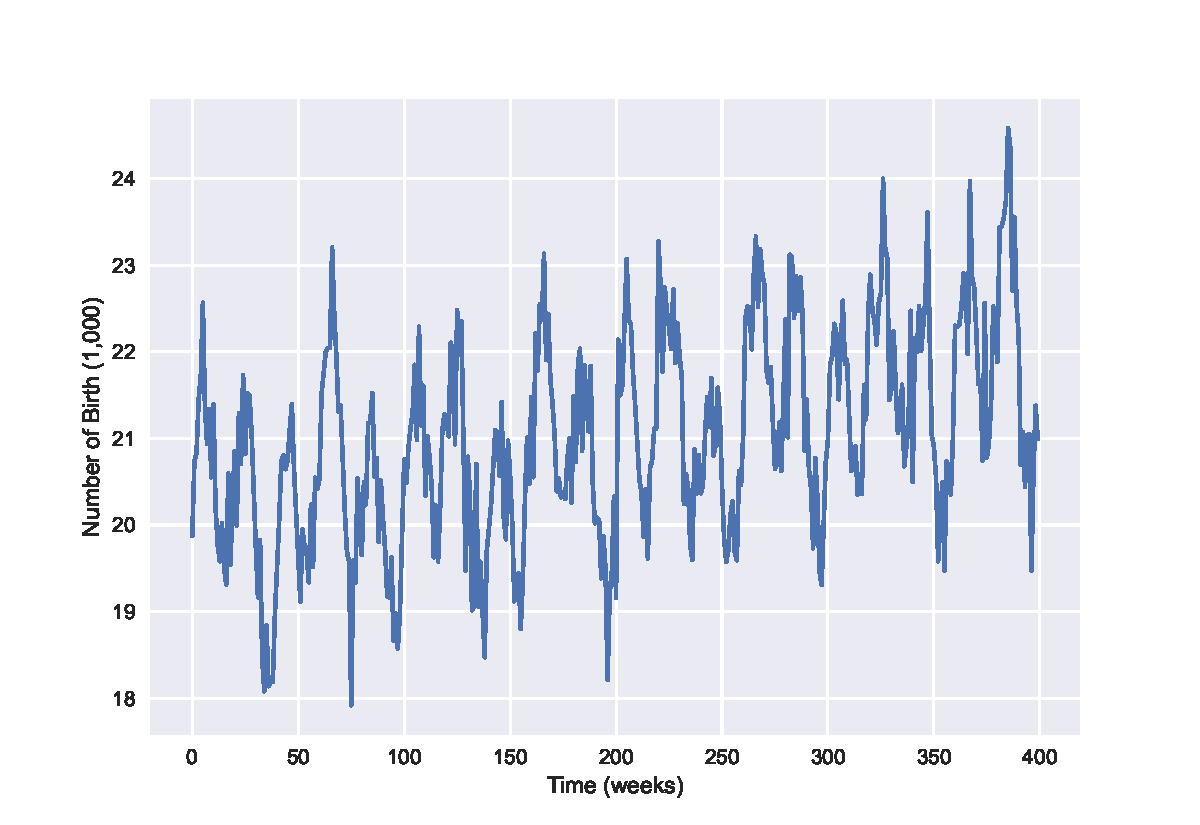
\includegraphics[width=0.8\linewidth]{graph1.pdf}
\end{center}
\end{figure}
We can see several patterns from the graph
\begin{itemize}
\item There is an overall trend of an increasing number of births over the sample period.
\item There is clear seasonality with a cycle approximately equal to 50 weeks. This cycle roughly corresponds to the calendar year as the peak of birth in March and October is consistently documented in the literature \citep{bobak2001seasonality,yang2021analysing}
\end{itemize}

For the following analysis, we split out data (400 observations in total) into training sample (the first 300 observations) and testing sample (the last 100 observations). For both STL and Bayesian models, we train the model with the training sample and then evaluate the model with both training sample and testing sample.

\section{Model and Results}
We would like to compare the performance of the traditional time series model and bayesian model. 

\subsection{STL Model}
Among numerous traditional time series forecasting model STL (Seaonsla and Trend decomposition using Loess\footnote{Loess is a method for estimating nonlinear relationships by doing local weighted regression}) \citep{cleveland1990stl} has been shown to be a robust versatile method with good performance in practice. 

\begin{align*}
	Y_t=T_t+S_t+R_t
\end{align*}

STL model basically assumes that the data $Y_t$ can be decomposed into three components, trend $T_t$, seasonal $S_t$ and remainder $R_t$ and the three components can be computed from the following steps \footnote{Here we only provide a naive STL implementation as the full model involves a lot of smoothing using local regression, moving average, adaptively adjusting weight. See \href{https://towardsdatascience.com/stl-decomposition-how-to-do-it-from-scratch-b686711986ec}{HERE} for more details. STL is already implemented in Python's statsmodels library}

\begin{itemize}
\item Find the approximate trend line fitting the time series data using, which can be obtained using OLS regression
\item Find the de-trended series by subtracting time series data with approximate trend line
\item Find the seasonal component by grouping the de-trended series by the cycle
\item Populate this component across the whole data
\item Find the de-seasonalized time series by subtracting time series data with seasonal data
\item Find the trend by fitting the de-seasonalized data to a polynomial model
\end{itemize}

By calling STL class in \emph{statsmodels} package, we get the following decomposition results\footnote{Note: the x-axis is only for calculation purpose as the STL model requires the index of series to be in Timestamp format. It is not the actual time of the data, which is omitted due to data usage restriction}:
\begin{figure}[H]
		\centering
	\caption{STL Decomposition}
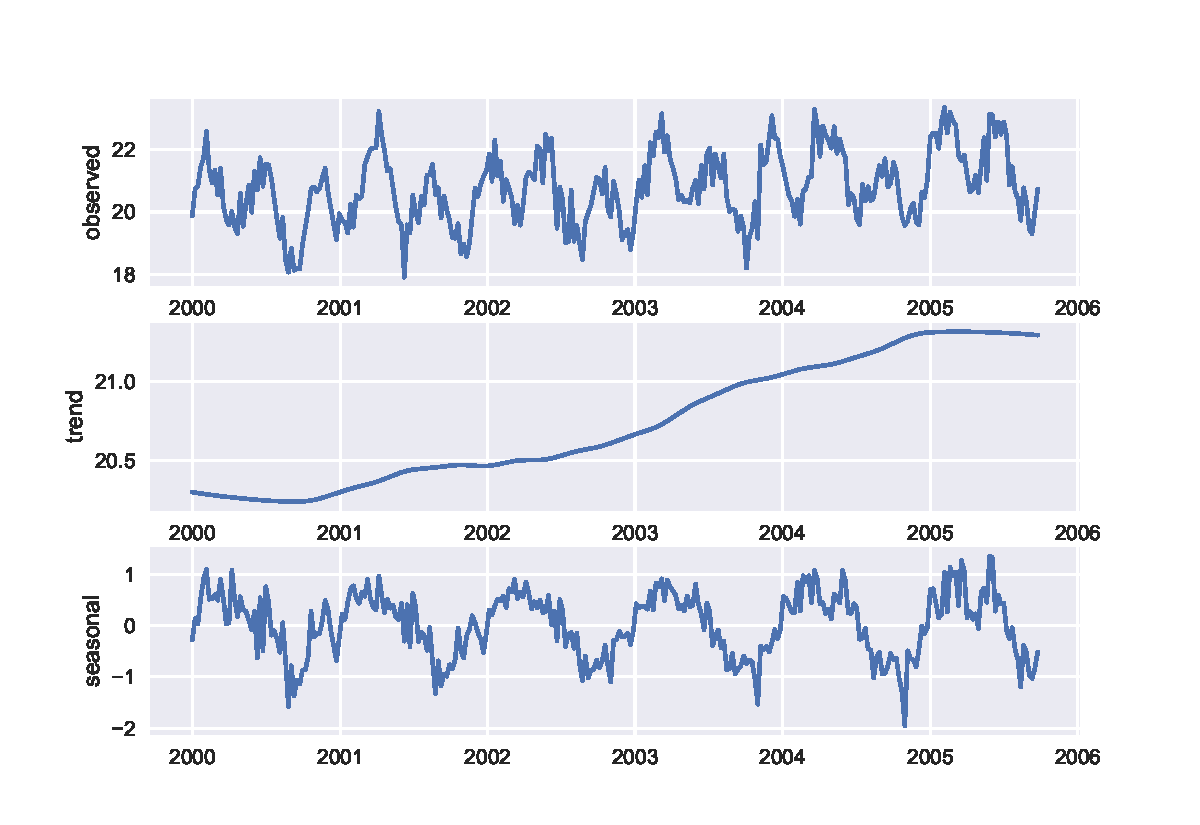
\includegraphics[width=\linewidth]{decompose.pdf}
\end{figure}

As we can see clearly from the above results: the overall trend is increasing and there is a strong seasonality with a cycle of approximately one year. \footnote{Based on the residual plot, there might be another seasonality component with a smaller cycle. However STL does not allow users to directly specify multiple seasonality components. We can probably work on this in the future to allow for more flexible multi-cycle structure} \\

We add the trend and seasonality component to get predictions from STL model, as presented below

\begin{figure}[H]
	\centering
	\caption{STL Model Prediction}
	\begin{subfigure}[h]{0.48\textwidth}
		\centering
		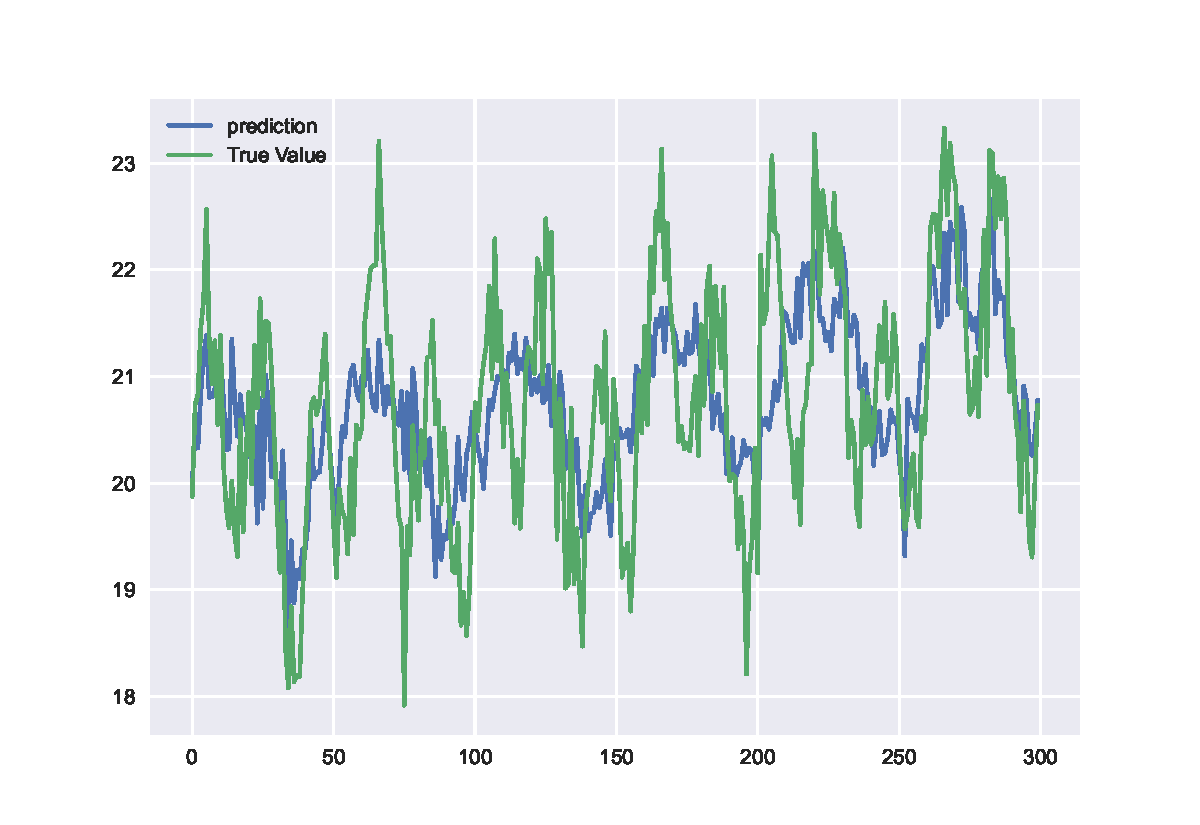
\includegraphics[width=\textwidth]{prediction_training.pdf}
		\caption{Training Sample}
	\end{subfigure}
	\begin{subfigure}[h]{0.48\textwidth}
		\centering
		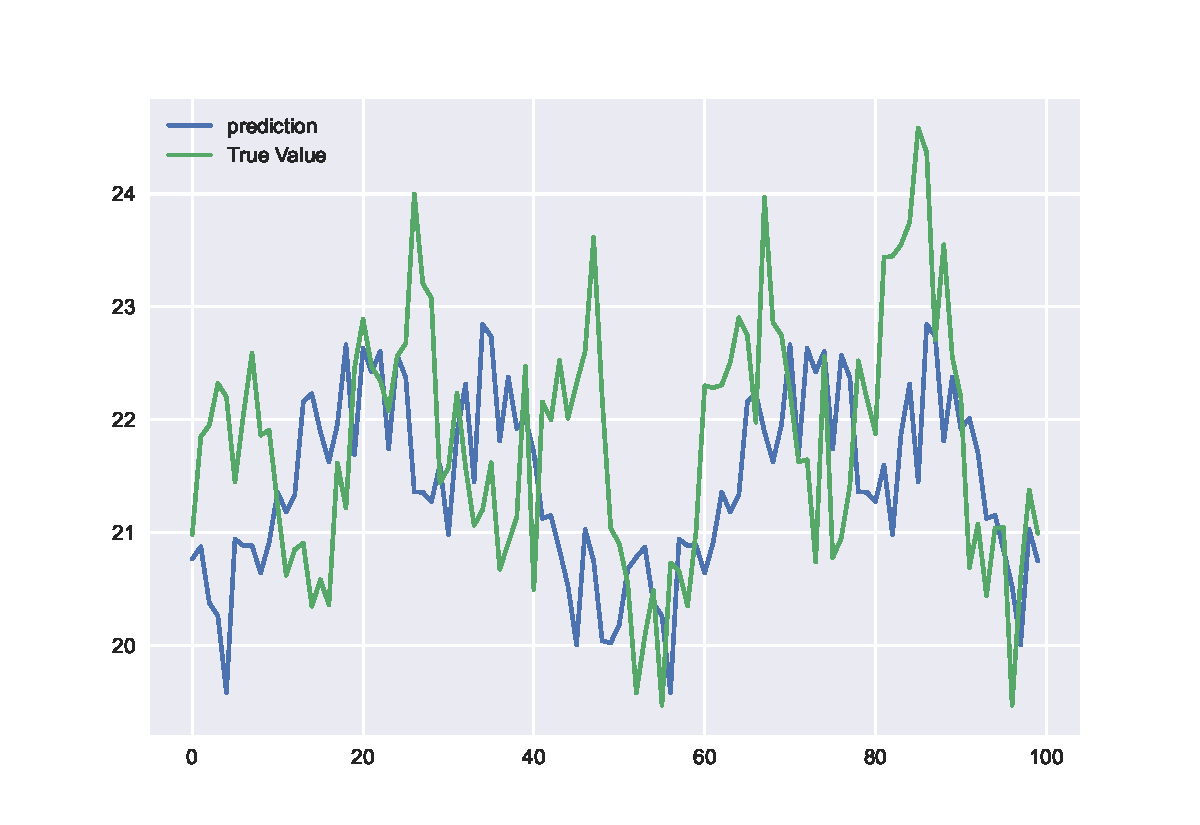
\includegraphics[width=\textwidth]{prediction_testing.pdf}
		\caption{Testing Sample}
	\end{subfigure}
	\label{match_map}
\end{figure}

\subsection{Bayesian Gaussian Process}
Guassian process is a stochastic process \footnote{A stochastic process is a (might be uncountable) collection of random variables along the (time) dimension} such that every finite collection of those random variables at different points of time has a multivariate normal distribution. The Gaussian Process problem is that:\\

We are given a time series $f(t)$ along the time dimension $t$, we want to make predictions $f(t')$ given some $t'$. The main estimation involves Bayesian updating (see \cite{williams2006gaussian} for more details, PyMC has already implemented this): suppose the prior distribution of $f(t)$ and $f(t')$ are given by 
\begin{align*}
f(t)&\sim N(\mu_{t},K_{t,t}) \\
f(t')&\sim N(\mu_{t'},K_{t',t'})
\end{align*}
Where $\mu_{t}$, $K_{t,t}$ are mean and variance functions evaluated at $t$ and  $\mu_{t'}$, $K_{t',t'}$ are the same functions evaluated at $t'$ . The join distribution of $(f(t),f(t'))$ is given by 
\begin{align*}
\begin{bmatrix} f(t)  \\ f(t')  \end{bmatrix}
\sim 
\mathbf{N}(\begin{bmatrix}
	\mu_{t} \\
	\mu_{t'}
\end{bmatrix}, 
\begin{bmatrix}
	K_{tt} & K_{tt'} \\
	K_{t't} & K_{t't'}
\end{bmatrix})
\end{align*}
Then based on Bayesian formula, the posterior distribution is given by 
\begin{align*}
f(t')|f(t)\sim \mathbf{N}(K_{t't}'K_{tt}^{-1}(f(t)-\mu_{t})+\mu_{t'},K_{t't'}-K_{tt'}'K_{tt}^{-1}K_{tt'})
\end{align*}

For Bayesian Gaussian process model, we specify the following model:
\begin{itemize}
\item Component 1 to capture the seasonality with cycle 52: periodic covariance function with lengthscale sampled from a \emph{Gamma(2,2)} prior distribution and period sampled from a \emph{Gamma(52,1)} prior distribution\footnote{Relatively informative prior is used based on our knowledge/literature}
\item Component 2 to capture the seasonality with the shorter cycle: periodic covariance function with lengthscale sampled from a \emph{Gamma(2,2)} prior distribution and period sampled from a \emph{Gamma(15,1)} prior distribution
\item Component 3 to capture the trend: linear covariance function with the constant term sampled from \emph{Normal(0.1,1)} distribution
\end{itemize} 

The results after updating is listed below:
\begin{table}[h]
	\begin{tabular}{llllllllll}
		\hline \hline
		& mean   & sd     & hdi\_2.5\% & hdi\_97.5\% & mcse\_mean & mcse\_sd & ess\_bulk & ess\_tail & r\_hat \\ \hline
		linear & 0.047  & 0.993  & -1.906     & 1.977       & 0.01       & 0.01     & 9900.0    & 6447.0    & 1.0    \\
		sns1   & 1.438  & 0.635  & 0.706      & 2.508       & 0.294      & 0.222    & 6.0       & 104.0     & 1.73   \\
		cycle1 & 78.138 & 25.967 & 51.67      & 104.971     & 12.956     & 9.923    & 6.0       & 112.0     & 1.73   \\
		sns2   & 1.662  & 0.232  & 1.198      & 2.095       & 0.018      & 0.012    & 170.0     & 5884.0    & 1.02   \\
		cycle2 & 20.009 & 0.026  & 19.956     & 20.059      & 0.0        & 0.0      & 8785.0    & 6239.0    & 1.0    \\
		sigma  & 0.492  & 0.021  & 0.451      & 0.531       & 0.0        & 0.0      & 9875.0    & 5924.0    & 1.0    \\ \hline \hline
	\end{tabular}
\end{table}

To make predictions, we sample 500 processes from the trace: the point prediction is calculated by taking the average of the 500 stochastic processes, the credible region of the process is obtained by taking the credible region at each individual time point. Predictions for the training sample and the testing sample are displayed below:
\begin{figure}[H]
	\centering
	\caption{Gaussian Process Prediction}
	\begin{subfigure}[h]{0.48\textwidth}
		\centering
		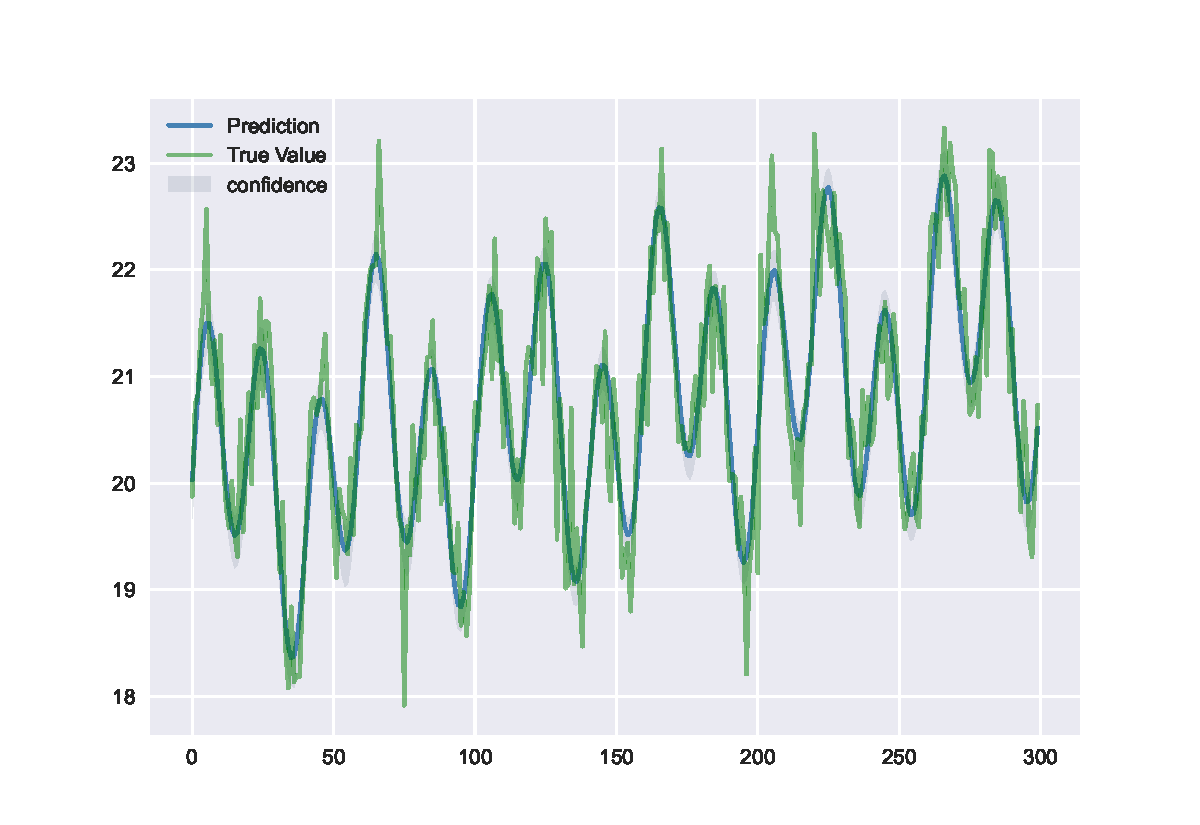
\includegraphics[width=\textwidth]{bayesian_prediction_training.pdf}
		\caption{Training Sample}
	\end{subfigure}
	\begin{subfigure}[h]{0.48\textwidth}
		\centering
		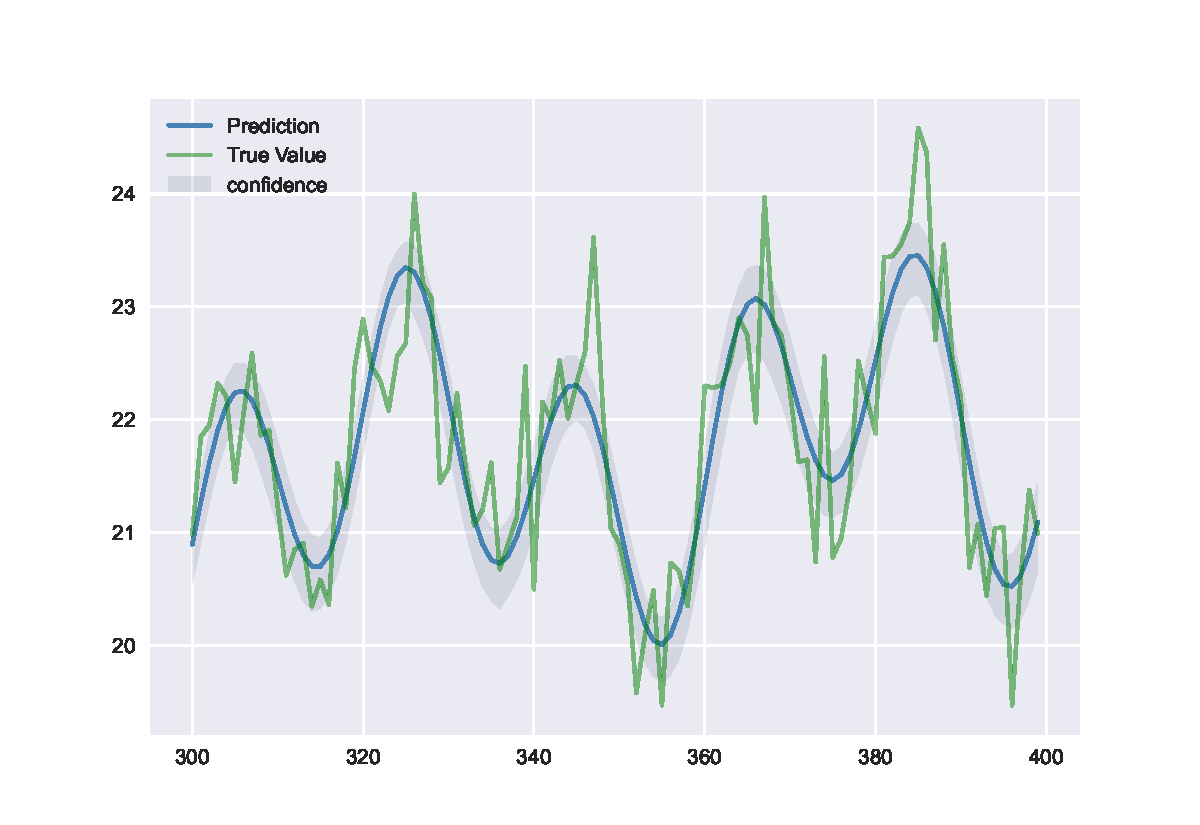
\includegraphics[width=\textwidth]{bayesian_prediction_testing.pdf}
		\caption{Testing Sample}
	\end{subfigure}
	\label{match_map}
\end{figure}

It is quite obvious that the Bayesian Gaussian Process approach generates better predictions based on a glance of the chart. To quantify the prediction accuracy, we calculate the $R^2$\footnote{For Bayesian Gaussian Process, we use the average of all sampling processes as our prediction} in the following table

\begin{table}[h]
	\centering
	\begin{tabular}{lll}
		\hline \hline
		& Training Sample     & Testing Sample    \\ \hline
		
		STL Model  & 0.418  & -0.318       \\  
		Bayesian Gaussian & 0.821 & 0.733 \\ \hline \hline
	\end{tabular}
\end{table}

As we can see from the table, the Bayesian Gaussian process model significantly outperforms the STL Model in both training sample and testing sample and the difference is even larger for testing sample (out of sample prediction)

\section{Conclusion}
From the analysis above, we can see that the Bayesian model significantly outperforms the traditional STL time series forecasting model with for both in and out of sample predictions and the difference is even larger for out of sample predictions. 

Of course, my conclusion only holds for this particular analysis and should be interpreted with caution. For future work, as we can see from the prediction residuals of STL model, there is still some kind of seasonality with a smaller cycle, we may choose to add another layer to further decompose the residual to improve the performance of this model, making the comparison more convincing. In addition, we can probably try to tune the parameters in both the STL and Bayesian Gaussian Process model to better fit data and generate better predictions. 


\clearpage
\setlength\bibsep{0pt}
\bibliographystyle{apalike}
\bibliography{document}

\newpage
\textbf{CODE}
\lstinputlisting[language=Python]{main.py}
\end{document}
